\chapter{Badania}\label{chap.research}
\section{Źródła danych}
Podczas badań zostały przeprowadzone testy wydajności dla trzech operacji, które są reprezentowane przez końcowy interfejs użytkownika. Dokładny opis dostępu do danych jak i ich struktury znajduje się w sekcji \ref{sec:twitter-api} oraz \ref{sec:tweet-structure}. Szczegółowa definicja operacji znajduję się w sekcji \ref{sec:user_interfaces}. 
Na potrzeby badań operacje nazwijmy następująco:
\begin{itemize}
	\item {Word Count}
	\item {Filter}
	\item {Reject}
\end{itemize}
Testy wydajności zostały wykonane na danych zebranych poprzez Twitter Developer API opisanym w sekcji \ref{sec:twitter-api}. Z racji iż strumieniowanie dla platformy Spark zapisuje dane cyklicznie, powstał katalog w systemie HDFS zawierający paczki danych zapisanych co 360 sekund. Na potrzeby badań wszystkie dane pobrane ze zdalnego API zostały połączone w jeden plik o wielkości \textbf{4GB}, który posłużył za źródło danych podczas wykonywania testów wydajności. Twitter Developer API nie jest standardowym webowym interfejsem typu REST\footnote{Representational state transfer}. Nie występuje tutaj standardowy scenariusz zapytanie do serwera, odpowiedź serwera. W przypadku danych strumieniowych, klient wysyła zapytanie do aplikacji, aplikacja wysyła zapytanie do serwerów Twitter i czeka na odpowiedź serwera asynchronicznie. Klient wysyłając jedynie żądanie nie blokuje samego interfejsu aplikacji. W związku z tym może występować złudzenie iż klient nie posiada kontroli nad samym pobieraniem danych, gdyż raz wysłane żądanie nie może zostać przerwane. Aplikacja sama zarządza procesem pobierania/strumieniowania danych. Architektura o podobnej strategii jest proponowana również przez twórców samego Twitter Developer API i jest zaprezentowana na pod adresem: \url{https://dev.twitter.com/streaming/overview}.
\begin{figure}
	\centering
	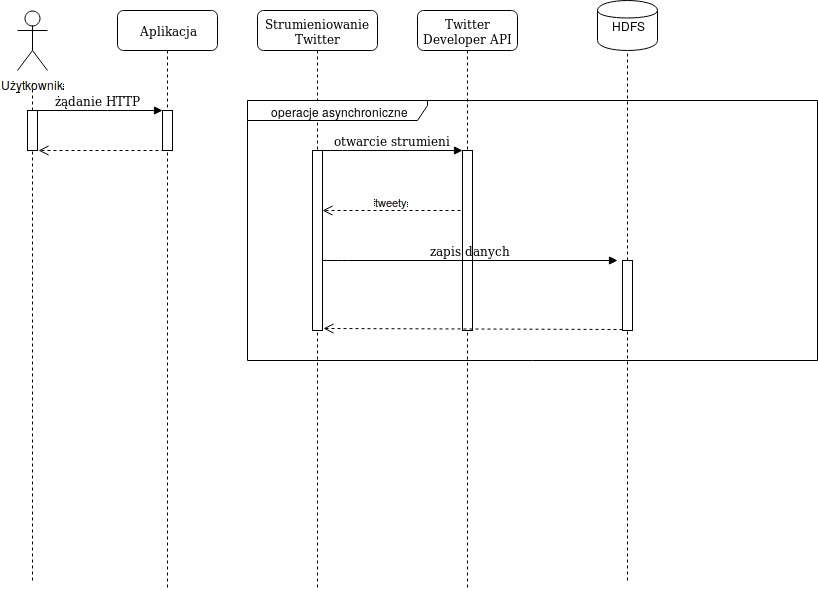
\includegraphics[scale=0.5]{twitter-api-connection.png}
	\caption{Architektura procesu pobierania danych z Twitter Developer API}
	\label{fig:@=twitter-api-connection}
\end{figure}
Proces strumieniowania danych z Twitter Developer API został przedstawiony na rysunku \ref{fig:@=twitter-api-connection}.
\section{Struktura źródeł danych}\label{sec:tweet-structure}
Dane pobrane z Twitter Developer API są zapisywane w systemie plików HDFS, który jest skonfigurowany z główną aplikacją. Dane są przyjmowane jako \textit{DStream}\footnote{Discretized Stream}, który jest główną warstwą abstrakcji dla strumieniowania danych. Wewnętrznie jest to ciąg stale napływających danych w formule RDD, szczegóły na temat RDD można znaleźć w sekcji\ref{rdd-section}. Następnie na napływających danych jest wywołana funkcja \textit{map}, która zapisuje równolegle rozproszony zbiór danych w systemie HDFS. Zapisanie jest dokonane w formacie JSON\footnote{JavaScript Object Notation}. JSON został wybrany ze względu na prostą strukturę i przystępną dla ludzkiego oka prezentację. Otwarcie strumieniowania jest przestawione w listingu \ref{lst:twitter-streaming-scala}  
\begin{lstlisting}[language=scala, caption={Otwarcie strumieniowania Twitter Developer API oraz zapis do HDFS},captionpos=b, label={lst:twitter-streaming-scala}]
val twitterInstance = new Twitter4JConfiguration(config).getTwitter4JAccess()
val tweetStream = TwitterUtils.createStream(SparkStreaming.streamingContext, Option(twitterInstance.getAuthorization)).map(new Gson().toJson(_))
tweetStream.foreachRDD((rdd, time) => {
val outputRDD = rdd.repartition(4)
outputRDD.saveAsTextFile(config.getString("hadoop-tweets-url").get + "tweet_" + time.milliseconds.toString)
})
SparkStreaming.streamingContext.start()
\end{lstlisting}
W linii nr 1 następuje konfiguracja dostępu do Twitter Developer API przy użyciu biblioteki Twitter4J\footnote{\url{http://twitter4j.org}}. Linia nr 2 to deklaracja strumienia, ustawienia autoryzacji dla Twitter Developer API oraz konfiguracja formatu zapisu danych. Linie nr 3,4,5 to konfiguracja samego zapisu w systemie HDFS, ustalana jest ilość partycji, na których ma zostać zapisane RDD oraz jak ma nazywać się wynikowy plik w HDFS. Linia nr 8 rozpoczyna faktyczne strumieniowanie danych oraz ich zapis.
\newline Struktura danych zwracana z Twitter Developer API w formacie JSON zawiera bardzo dużo informacji. Jedne z najbardziej kluczowych są przedstawione w liście \ref{items:tweet-fields}
\begin{itemize}\label{items:tweet-fields}
	\item Data utworzenia\footnote{createdAt}
	\item Udostępnienia tweet'a \footnote{retweetedStatus}
	\item Zawartość tweet'a\footnote{text}
	\item Autor\footnote{user}
	\item Flaga prawda/fałsz dotycząca treści wrażliwych\footnote{isPossiblySensitive}
\end{itemize}
Dokładna struktura danych jest przedstawiona w listingu: \ref{lst:tweet-json}
\lstinputlisting[language=json,firstnumber=1, label={lst:tweet-json}, captionpos=b, caption={Przykładowa struktura danych pobrana z Twitter Developer API, użyta podczas badań.}]{tweet.json}  
\section{Specyfikacja sprzętowa i konfiguracja platform}
Badania zostały przeprowadzone na maszynie o specyfikacji:
\begin{itemize}
	\item Procesor: Intel Core i7-4702MQ (2.2GHz Quad-core + HT) 
	\item Pamięć RAM: 16GB
	\item Pamięć masowa: 1 TB 5400rpm\footnote{Revolutions per minute - obroty na minutę} SATA
	\item Karta graficzna: NVIDIA GeForce GT 750M (2G)  
\end{itemize}
Podczas badań specyfikacja karty graficznej nie ma wpływu na wyniki, gdyż dla badanych operacji wykorzystywane są trzy jednostki obliczeniowe: procesor, pamięć RAM, dysk twardy.
\newline Pomiary wydajności zostały dokonane przy pomocy programu \textbf{cURL}.\footnote{\url{https://curl.haxx.se/}} Testy obejmują siedem następujących czynników:
\begin{itemize}\label{items:time-descriptions}
	\item{Czas rozwiązywania adresu\footnote{time\_namelookup}}
	\item{Czas połączenia TCP\footnote{time\_connect}}
	\item{Czas wymiany informacji między połączeniami (handshake)\footnote{time\_appconnect}} 
	\item{Czas całkowity przed wymianą informacji\footnote{time\_pretransfer}}
	\item{Czas przekierowań\footnote{time\_redirect}}
	\item{Czas przed którym pierwszy bajt danych miał zostać wysłany\footnote{time\_starttransfer}}
	\item{Czas całkowity\footnote{time\_total}}
\end{itemize}
Obydwie platformy pozwalają na szczegółową konfigurację instalacji. Z racji iż testy były wykonywane na jednej i tej samej maszynie należało ustawić sztuczny(wirtualny) klaster. Oznacza to, że na maszynie było imitowane rozproszone środowisko obliczeniowe. Dla Apache Spark tryb lokalny został ustawiony na maksymalną możliwą liczbę dostępnych wątków wirtualnej maszyny Java - oznacza to, że liczba zwróconych dostępnych wątków przez metodę przedstawioną na listingu \ref{lst:jvm-threads-access} definiuje ile operacji Apache Spark może wykonywać w tej samej jednostce czasu. Konfiguracja jest widoczna na listingu \ref{lst:spark-cluster-config}. Konfiguracja pozwala na tworzenie kontekstu dla zapytań o dane statyczne (na przykład baza danych), jak również o charakterze dynamicznym (strumieniowanie). Jak widać na listingu \ref{lst:spark-cluster-config} w linii 4 ustawiany jest również cykl zapisu danych dynamicznych (zapis co 360 sekund).
\begin{lstlisting}[language=scala, caption={Metoda zwracająca liczbę dostępnych wątków wirtualnej maszyny Java},captionpos=b, label={lst:jvm-threads-access}]
Runtime.getRuntime.availableProcessors() 
\end{lstlisting}
\begin{lstlisting}[language=scala, caption={Konfigracja klastra dla Apache Spark},captionpos=b, label={lst:spark-cluster-config}]
object SparkStreaming {
val conf = new SparkConf().setMaster("local[*]").setAppName("big-data-runner-spark-driver-application")
val sparkContext = new SparkContext(conf)
val streamingContext = new StreamingContext(sparkContext, Seconds(360))
}
\end{lstlisting} 
Apache Hadoop może być uruchamiany w trzech trybach: pojedynczy proces JVM (\textit{Standalone Operation)}, pseudo rozproszony \textit{Pseudo-Distributed Operation}, w pełni rozproszony \textit{Fully-Distributed Operation}. Aby konfiguracja była jak najbardziej podobna do konfiguracji Spark, Hadoop został uruchomiony w trybie pseudo rozproszonym. W takim przypadku Apache Hadoop nie jest konfigurowany przez kod źródłowy, lecz przez pliki konfiguracyjne XML. Konfiguracja Apache Hadoop jest przedstawiona na listingach \ref{lst:core-site} i \ref{lst:hdfs-site}.
\begin{lstlisting}[language=XML, label={lst:hdfs-site},captionpos=b, caption={Konfigracja Apache Hadoop dla trybu pseudo rozproszonego. Plik hdfs-site.xml}]
<configuration>
	<property>
		<name>dfs.replication</name>
		<value>4</value>
	</property>
</configuration>
\end{lstlisting}
\begin{lstlisting}[language=XML, label={lst:core-site}, captionpos=b, caption={Konfigracja Apache Hadoop dla trybu pseudo rozproszonego. Plik core-site.xml}, float]
<configuration>
	<property>
		<name>fs.defaultFS</name>
		<value>hdfs://127.0.0.1:8080</value>
	</property>
	<property>
		<name>hadoop.tmp.dir</name>
		<value>/home/szymonidas/tweets-hdfs/</value>
	</property>
</configuration>
\end{lstlisting}
Poza adresem Apache Hadoop, został zdefiniowany katalog na dysku twardym, gdzie HDFS będzie przechowywał swoje dane. Hadoop podobnie jak Spark został ustawiony na partycjonowanie danych w czterech częściach.
\section{Wyniki}
Dla operacji \textit{Word Count} wyniki wydajności są przedstawione w tabeli \ref{tab:word-count-results}. Wielkość pliku wsadowego to 4 GB. Można zaobserwować, że operacja na platformie Apache Spark jest około cztery razy szybsza od Apache Hadoop. Wszystkie pomiary poza $time\_starttransfer$ oraz $time\_total$ można uznać za pomijalne dla końcowego użytkownika. Warto też odnotować iż operacja \textit{Word Count} jest najbardziej czasochłonną operacją spośród wszystkich badanych.  
\begin{table}[]
	\centering
	\caption{Wyniki wydajności dla zliczania ilości wystąpień poszczególnych fraz tekstowych (oddzielonych spacją) znalezionych w źródle danych oraz zapisu wyniku do pliku}
	\label{tab:word-count-results}
	\begin{tabular}{|l|l|l|}
		\hline
		Czas [s]    & Hadoop     & Spark      \\ \hline
		time\_namelookup    & 0.000020   & 0.000023   \\ \hline
		time\_connect       & 0.000097   & 0.000116   \\ \hline
		time\_appconnect    & 0.000000   & 0.000000   \\ \hline
		time\_pretransfer   & 0.000116   & 0.000134   \\ \hline
		time\_redirect      & 0.000000   & 0.000000   \\ \hline
		time\_starttransfer & 402.792577 & 111.232410 \\ \hline
		time\_total         & 402.792625 & 111.232446 \\ \hline
	\end{tabular}
\end{table}
\newline Dla operacji \textit{Filter} wyniki wydajności są przedstawione w tabeli \ref{tab:filter-results}. Wielkość pliku wsadowego to 4GB. Operacja \textit{Filter} jest około dwa i pół raza wolniejsza na platformie Apache Hadoop w stosunku do Apache Spark. Również w tym przypadku wszelkie pomiary poza $time\_starttransfer$ oraz $time\_total$ można uznać za pomijalne dla końcowego użytkownika. Operacja \textit{Filter} jest najkrócej trwającą, ze wszystkich badanych. 
\begin{table}[]
	\centering
	\caption{Wyniki wydajności dla zliczania ilości linii zawierających frazę tekstową zdefiniowaną przez użytkownika}
	\label{tab:filter-results}
	\begin{tabular}{|l|l|l|}
		\hline
		Czas [s]    & Hadoop    & Spark     \\ \hline
		time\_namelookup    & 0.000022  & 0.000029  \\ \hline
		time\_connect       & 0.000090  & 0.000113  \\ \hline
		time\_appconnect    & 0.000000  & 0.000000  \\ \hline
		time\_pretransfer   & 0.000110  & 0.000140  \\ \hline
		time\_redirect      & 0.000000  & 0.000000  \\ \hline
		time\_starttransfer & 42.685888 & 16.489812 \\ \hline
		time\_total         & 42.685924 & 16.489860 \\ \hline
	\end{tabular}
\end{table}
\newline Dla operacji \textit{Reject} wyniki wydajności są przedstawione w tabeli \ref{tab:reject-results}. Wielkość pliku wsadowego to 4GB. Operacja \textit{Reject} jest około pięciu razy szybsza dla platformy Apache Spark w stosunku do Apache Hadoop. Tak jak w dwóch poprzednich badanych przypadkach: \textit{Filter} oraz \textit{Word Count} pomiary poza $time\_starttransfer$ oraz $time\_total$ można uznać za pomijalne dla końcowego użytkownika.
\begin{table}[]
	\centering
	\caption{Wyniki wydajności odrzucenia linii zawierających frazę tekstową zdefiniowaną przez użytkownika oraz zapisania wyniku do pliku}
	\label{tab:reject-results}
	\begin{tabular}{|l|l|l|}
		\hline
		Czas [s]    & Hadoop     & Spark     \\ \hline
		time\_namelookup    & 0.000025   & 0.000049  \\ \hline
		time\_connect       & 0.000098   & 0.000184  \\ \hline
		time\_appconnect    & 0.000000   & 0.000000  \\ \hline
		time\_pretransfer   & 0.000118   & 0.000237  \\ \hline
		time\_redirect      & 0.000000   & 0.000000  \\ \hline
		time\_starttransfer & 238.408629 & 45.186254 \\ \hline
		time\_total         & 238.408673 & 45.186296 \\ \hline
	\end{tabular}
\end{table}
\section{Interpretacja wyników}
Z punktu widzenia badanej wydajności wszystkie pomiary poza \textbf{time\_starttransfer} oraz \textbf{time\_total} nie są kluczowe gdyż pomijają czas pracy badanych platform. Czas całkowity jest interesujący z punktu widzenia użytkownika systemu, którego interesuje faktyczny czas uzyskania wyników. Podczas interpretacji wyników mylący może być opis przedstawiony w \ref{items:time-descriptions} \textit{Czas przed którym pierwszy bajt danych miał zostać wysłany}. Opis ten nie dotyczy danych, które są przetwarzane na badanych platformach lecz danych wysłanych przez odpowiedź na żądanie HTTP. Oznacza to, że dane odpowiedzi zostały wysłane po czasie gdy wszystkie obliczenia na platformie zostały już wykonane. W związku z tym \textbf{time\_starttransfer} może zostać uznany za czas pracy przetwarzania na danej platformie.
\newline W związku z wynikami przedstawionymi w tabelach \ref{tab:filter-results}, \ref{tab:reject-results}, \ref{tab:word-count-results} możemy zaobserwować zależność, że platforma Spark jest zdecydowanie szybsza (od dwóch i pół do pięciu razy) jeżeli chodzi o wykonywanie obliczeń i zapis wyników do pliku w systemie HDFS. Porównanie wydajności wszystkich operacji jest przedstawione na \ref{fig:results-comparison-bar}
\begin{figure}[!htb]
	\centering
	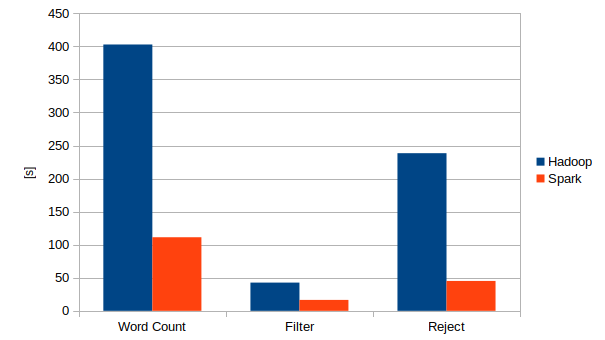
\includegraphics[scale=0.6]{results-comparison-bar.png}
	\caption{Wyniki wydajności operacji: Word Count, Filter i Reject na platformach Apache Spark oraz Apache Hadoop.}
	\label{fig:results-comparison-bar}
\end{figure}   
\section{Koszty rozwoju oprogramowania i zasobów ludzkich}
Badane platformy Apache Spark oraz Apache Hadoop są przedstawicielami dwóch języków programowania dedykowanych na platformę JVM: Scala oraz Java. Apache Spark jest narzędziem napisanym w języku Scala i posiada interfejs programistyczny dla czterech języków programowania: Scala, Java, Python oraz R. Apache Hadoop to narzędzie oparte wyłącznie na języku Java. Rozwijanie systemów informatycznych wiąże się z wieloma aspektami takimi jak: koszty rekrutacji inżynierów posiadających wiedzę z wąskiej dziedziny np. język programowania, ramy projektowej, poszczególnych bibliotek. Innym aspektem długofalowego projektu informatycznego jest pozostawienie możliwości na rozszerzanie rozwiązania oraz integracja z innymi platformami bądź językami programowania. W przypadku Apache Hadoop rozwiązanie jest zamknięte na język Java i integracja z innymi językami programowania wymaga serializacji danych bądź też ich zapisu we wcześniej uzgodnionym formacie na przykład HDFS. W przypadku Apache Spark prace implementacji systemu mogą być prowadzone w kilku językach. Dodatkowo można wykorzystywać zaletę samego języka Scala, gdzie wszystkie biblioteki z języka Java są dostępne i nie wymagają żadnego dodatkowego nakładu pracy przy ich użyciu. W kontekście tej pracy magisterskiej zostały wykonane implementacje tych samych funkcjonalności dla dwóch języków Scala i Java. Operacja zliczenia wystąpień danej frazy w linii dla języka Scala została przedstawiona w listingu \ref{lst:scala-occurence-listing}. Ta sama operacja dla języka Java została przedstawiona w listingu \ref{lst:java-occurrence-listing}.
\begin{lstlisting}[language=scala, caption={Operacja zliczania wystąpień danej frazy w linii dla języka Scala na platformie Apache Spark},captionpos=b, label={lst:scala-occurence-listing}]
class WordOccurrence {
	def run(sparkContext: SparkContext, filePath: String, word: String) = {
	val lines: RDD[String] = sparkContext.textFile(filePath)
	val linesContainingWord = lines.filter(line => line.contains(word))
	linesContainingWord.count()
	}
}
\end{lstlisting}
\begin{lstlisting}[language=Java, caption={Operacja zliczania wystąpień danej frazy w linii dla języka Java na platformie Apache Hadoop},captionpos=b, label={lst:java-occurrence-listing}]
public class WordOccurrence {

public long run(String basePathHDFS, String wordToBeFound) throws Exception {
Path pt = new Path(basePathHDFS + "mergedTweets0.3686418061949279.txt");
Configuration conf = new Configuration();
conf.set("fs.defaultFS", basePathHDFS);
conf.set("wordToBeFound", wordToBeFound);
Job job = new Job(conf, "WordOccurrence");
job.setOutputKeyClass(Text.class);
job.setOutputValueClass(IntWritable.class);

job.setMapperClass(FilterMapper.class);
job.setReducerClass(SimpleReduce.class);

job.setInputFormatClass(TextInputFormat.class);
job.setOutputFormatClass(TextOutputFormat.class);

FileInputFormat.addInputPath(job, pt);
TimeStamp myTs = TimeStamp.getCurrentTime();
FileOutputFormat.setOutputPath(job, new Path(basePathHDFS + "hadoopWordOccurrenceResult" + myTs));
job.waitForCompletion(true);
return job.getCounters().findCounter("org.apache.hadoop.mapred.Task$Counter", "MAP_OUTPUT_RECORDS").getValue();
}

}

public class FilterMapper extends Mapper<LongWritable, Text, Text, IntWritable> {
private final IntWritable one = new IntWritable(1);
private Text word = new Text();

public void map(LongWritable key, Text value, Context context) throws IOException, InterruptedException {
String wordToBeFound = context.getConfiguration().get("wordToBeFound");
String line = value.toString();
if (line.contains(wordToBeFound)) {
context.write(word, one);
}
}
}
public class SimpleReduce extends Reducer<Text, IntWritable, Text, IntWritable> {
public void reduce(Text key, Iterable<IntWritable> values, Context context)
throws IOException, InterruptedException {
int sum = 0;
for (IntWritable val : values) {
sum += val.get();
}
context.write(key, new IntWritable(sum));
}
}
\end{lstlisting}
Nie trudno zauważyć, że ta sama funkcjonalność dla języka Scala może być przedstawiona o wiele bardziej zwięźle i czytelnie niż w języku Java. Sama różnica w ilości kodu jest zauważalna - Scala 7 linii, Java 48 linii. W przypadku utrzymywania kodu jest to bardzo ważne by rozwiązania były czytelne i łatwe do opanowania. Szczególnie istotne jest to w dużych projektach, gdzie inżynierowie często zmieniają odpowiedzialność za dany fragment funkcjonalności, bądź też występuje duża rotacja programistów. Wybór języka programowania, może też mieć znaczący wpływ na koszty rozwoju oraz utrzymania danego projektu informatycznego z racji na różnice w zarobkach ze względu na technologię. Na wykresach \ref{fig:@=salaries_contract} oraz \ref{fig:@=salaries_permanent} możemy zobaczyć koszty zatrudniania inżynierów ze względu na technologię oraz rodzaj zatrudnienia w latach 2015, 2016 oraz 2017 na terenie Wielkiej Brytanii. Dane zostały pobrane z serwisu internetowego \url{https://www.itjobswatch.co.uk}.
\begin{figure}[h]
	\centering
	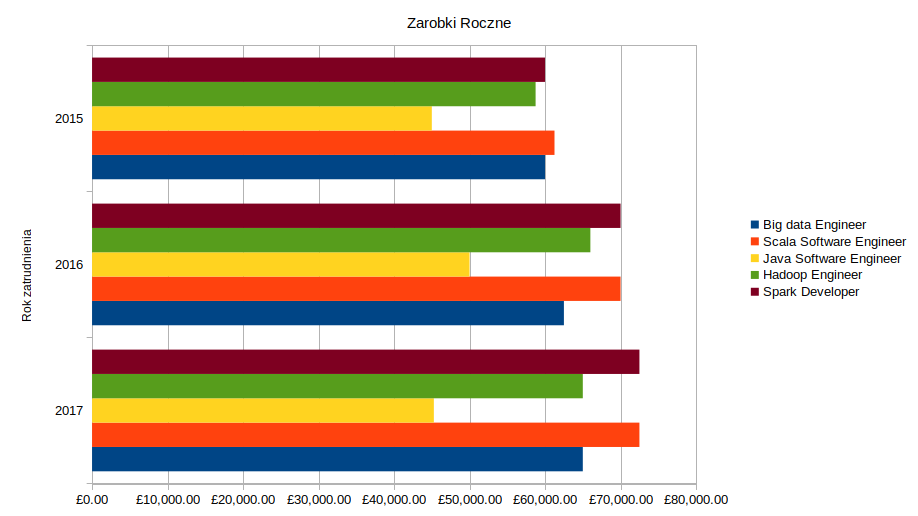
\includegraphics[scale=0.5]{salaries_contract.png}
	\caption{Trendy zarobków rocznych na terenie Wielkiej Brytanii w latach 2015, 2016 oraz 2017 dla formy zatrudnienia na kontrakt.}
	\label{fig:@=salaries_contract}
\end{figure}
\begin{figure}[h]
	\centering
	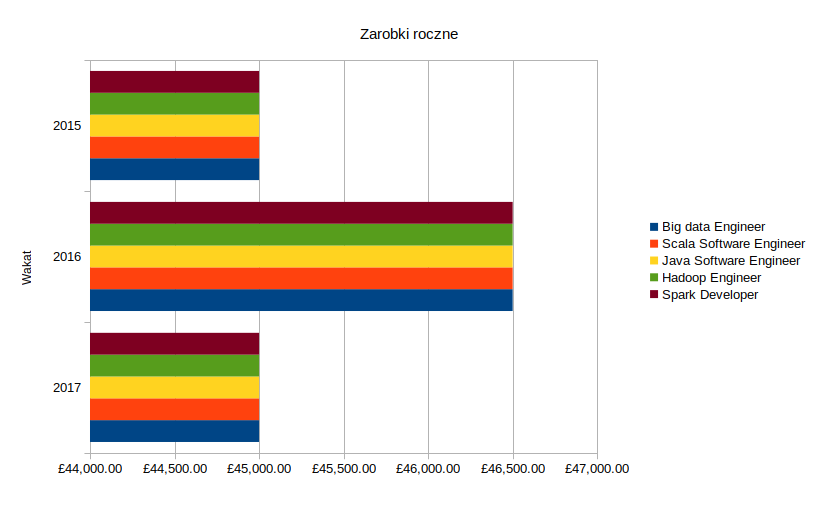
\includegraphics[scale=0.5]{salaries_permanent.png}
	\caption{Trendy zarobków rocznych na terenie Wielkiej Brytanii w latach 2015, 2016 oraz 2017 dla formy zatrudnienia stałego (umowy o pracę).}
	\label{fig:@=salaries_permanent}
\end{figure}
\newline Na podstawie rysunku \ref{fig:@=salaries_permanent} możemy zauważyć, że w kontekście rekrutacji ze względu na narzędzie bądź język programowania nie występują różnice płac dla stałej formy zatrudnienia. Jest to szczególnie istotne dla projektów o charakterystyce długofalowej oraz dużej wielkości. W przypadku formy zatrudniania stałego pracowników i dużych projektach można wybrać dowolną technologię, gdyż koszty będą relatywnie takie same (wyniki to średnie płac na dane stanowisko). Przedsiębiorstwo może również wybrać tą technologię bądź język programowania, który jest opanowany przez największą grupę docelową na rynku pracy tak by zwiększyć swoje możliwości rekrutacyjne.\newline Zupełnie odwrotnie przedstawia się sytuacja dla okresowej formy zatrudnienia tak zwany kontrakt. Dokładne dane dotyczące formy zatrudnienia na kontrakt są widoczne na rysunku \ref{fig:@=salaries_contract}. Można zaobserwować zróżnicowane płac rocznych ze względu na narzędzie bądź język programowania sięga dwudziestu siedmiu i pół tysiąca funtów rocznie. W ostatnich trzech latach najtańsze były osoby zatrudnione na kontrakt znające język programowania Java. Drugie miejsce od końca najwyższych płac rocznych zajmują inżynierowie znający Apache Hadoop. Najdroższe osoby to te posiadające kompetencje w platformie Apache Spark. 